\RequirePackage{luatex85}
\documentclass{standalone}
\usepackage{tikz}

% Color Definitions
\definecolor{SourceColor}{RGB}{85,168,104}
\definecolor{TargetColor}{RGB}{221,132,82}
\definecolor{TargetChangerColor}{RGB}{255,153,0}
\definecolor{AbsorbingAreaColor}{RGB}{196,78,82}
\definecolor{ObstacleColor}{RGB}{179,179,179}
\definecolor{StairColor}{RGB}{129,114,178}
\definecolor{MeasurementAreaColor}{RGB}{255,0,0}
\definecolor{InformationAreaColor}{RGB}{0,100,20}
\definecolor{AerosolCloudColor}{RGB}{202,156,76}
\definecolor{AgentColor}{RGB}{76,114,202}
\definecolor{AgentIdColor}{RGB}{255,127,0}

\newcommand{\MeasurementAreaOpacity}{0.549020}
\newcommand{\AerosolCloudOpacity}{0.039216}
\usetikzlibrary{shapes,arrows,chains}


\begin{document}

\begin{tikzpicture}
\node[] at (-1.8,0) { 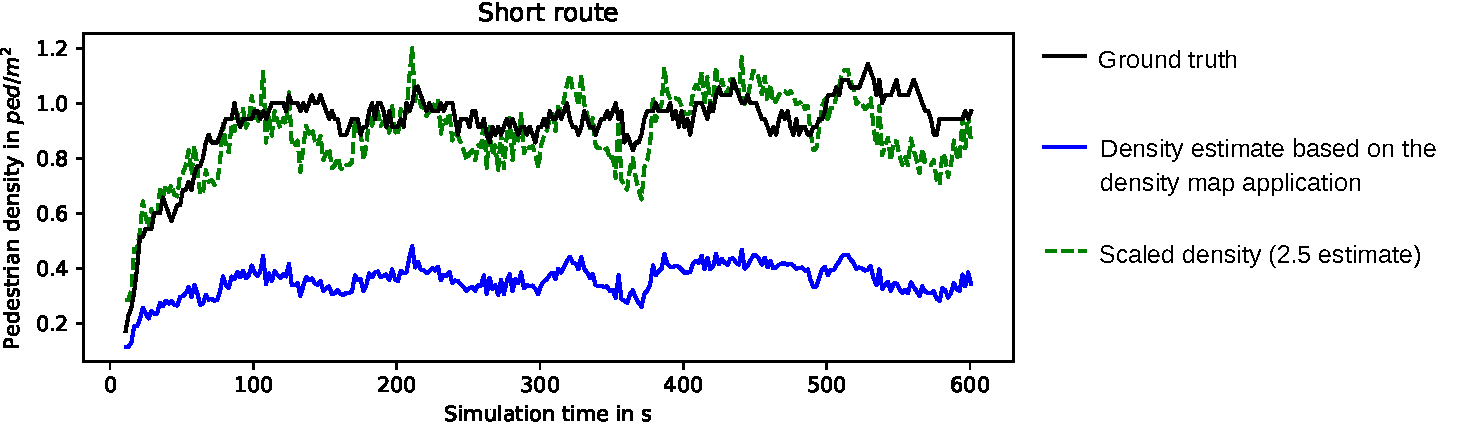
\includegraphics[height=5cm, trim={0 0 7.5cm 0}, clip]{./ShortRoute.pdf}};
\node[] at (0,-5.5) { 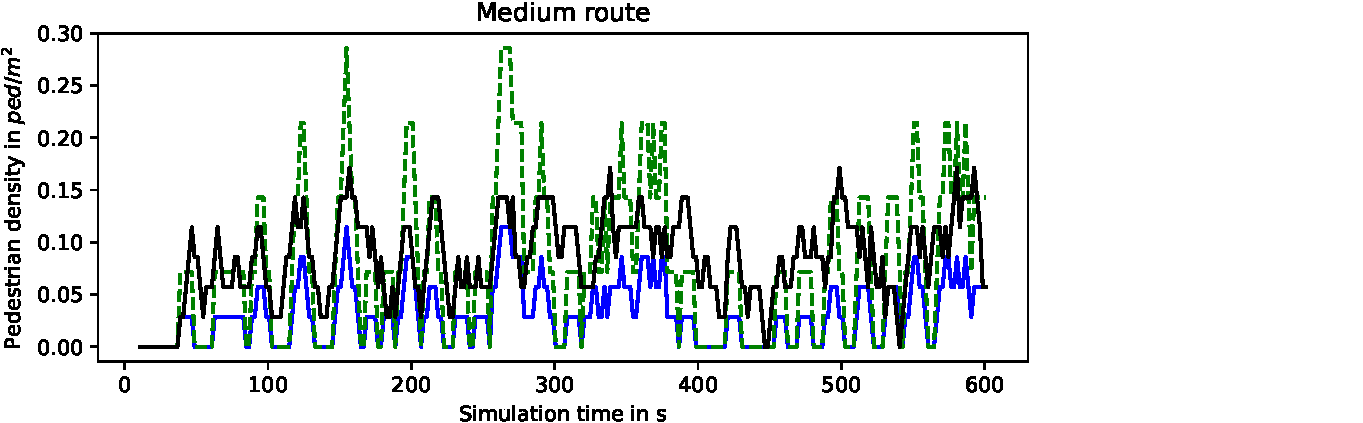
\includegraphics[height=5cm]{./MediumRoute.pdf}};
\node[] at (0,-11) { 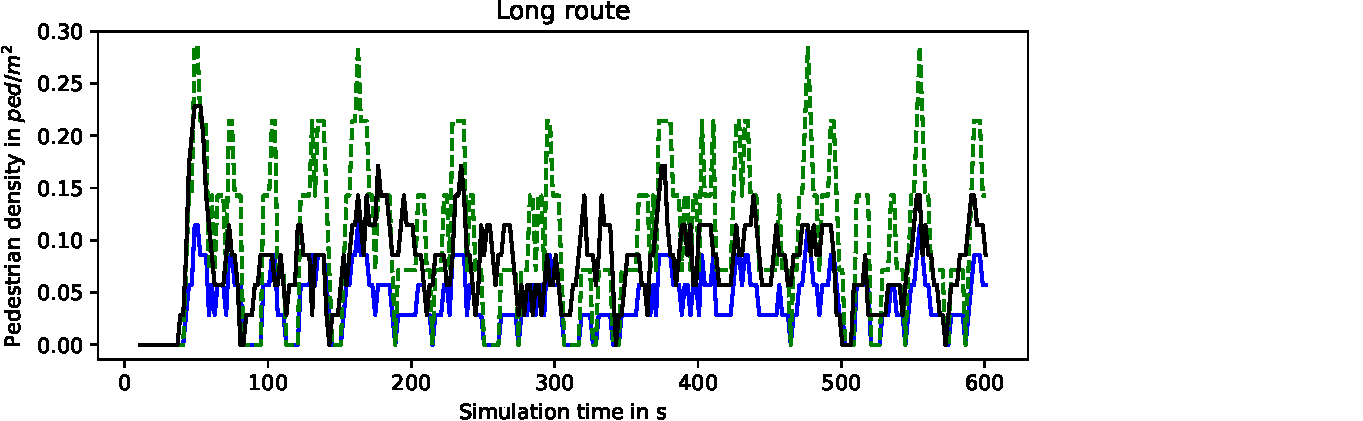
\includegraphics[height=5cm]{./LongRoute.pdf}};
\node[text width=3cm] at (7,-3.3) { Ground truth};
\node[text width=3cm] at (7,-5.9) { Systematically underestimated density (density map application)};
\node[text width=3cm] at (7,-7.6) { Scaled estimate (factor: 2.5)};
\node[] at (0,-18) { 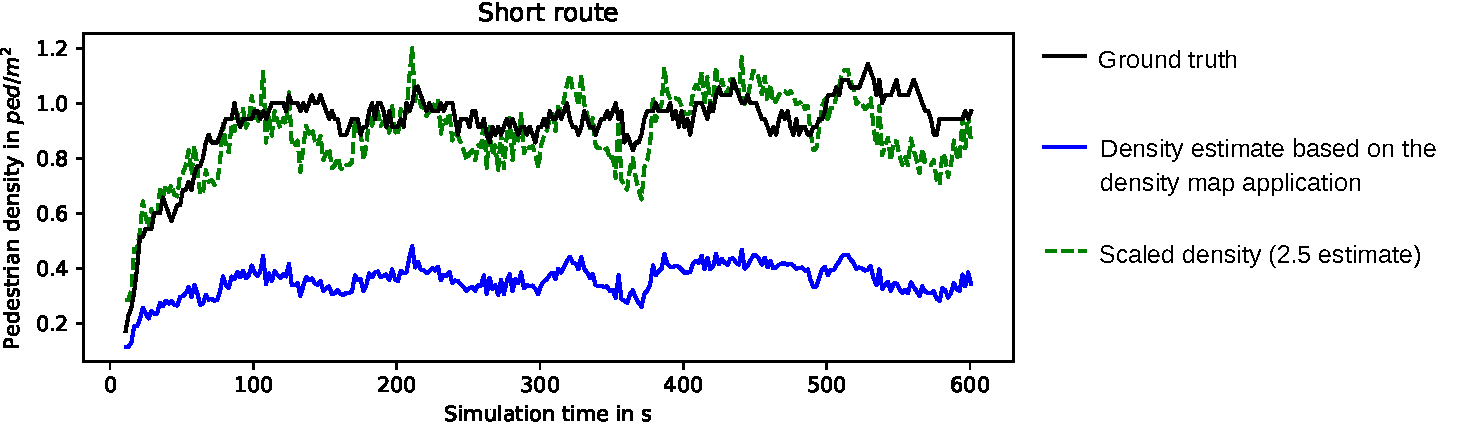
\includegraphics[width=0.85cm, trim={17.7cm 1cm 6.4cm 0}, clip]{./ShortRoute.pdf}};



\end{tikzpicture}
\end{document}
